\documentclass[10pt,twocolumn]{article}
\usepackage[utf8]{inputenc}
\usepackage[T1]{fontenc}
\usepackage[english]{babel}
\usepackage[a4paper,margin=2cm]{geometry}
\usepackage{amsmath,amssymb}
\usepackage{graphicx}
\usepackage{booktabs}
\usepackage{hyperref}
\usepackage{xcolor}
\usepackage{natbib}
\bibliographystyle{plainnat}
\usepackage{caption}
\captionsetup{font=small, labelfont=bf}
\usepackage[capitalise,noabbrev]{cleveref}
\newcommand{\dd}{\mathrm{d}}

\hypersetup{colorlinks=true, linkcolor=blue!50!black, citecolor=blue!50!black,
  urlcolor=blue!50!black}

\title{\bfseries HotCarWatch:\\
  A free, no-login physical decision-support tool\\
  for vehicular hyperthermia in children and pets}
\author{
  Anonymous Authors\\
  \texttt{\small hotcarwatch.local}
}
\date{May 2026}

\begin{document}
\twocolumn[
\begin{@twocolumnfalse}
\maketitle
\begin{abstract}
\noindent
Since 1998, 1\,047 US children have died of vehicular hyperthermia
(NoHeatstroke.org, Jan Null SJSU); an additional several hundred
pets die in parked cars each summer.  All of these deaths are
preventable.  \citet{mclaren2005pediatrics} established that the
cabin of a parked car rises $\approx$\,22\,$^\circ$C above ambient
within 60\,min and that 80\% of the rise occurs in the first
30\,min, independently of the outdoor temperature.  Yet the average
parent does not have a calibrated, on-the-spot tool to translate
``it's 27\,$^\circ$C outside; I'll be back in 15 minutes'' into the
predicted cabin and core-body temperatures.  We present
\textsc{HotCarWatch}, an open-source cabin lumped-capacitance
thermal-balance model coupled to a simplified occupant
core-body-temperature ODE, packaged as a public-domain Python
library and an entirely client-side web frontend.  Validation
against \citet{mclaren2005pediatrics} and \citet{vanos2018temperature}
yields 16/16 cases within tolerance.  Across the four scenarios
$\times$ seven vehicles $\times$ eight occupants tested, the only
intervention that prevented heat injury in 100\% of cases was
\emph{do not leave the occupant in the vehicle}.  The frontend
($\approx$\,8.8\,KB gzipped) runs in any browser with no backend,
no login, and no data collection, and is deployable at \$0 operating
cost.
\end{abstract}
\vspace{1em}
\end{@twocolumnfalse}
]

\section{Introduction}

Pediatric vehicular hyperthermia is among the most preventable
causes of child death in the United States.
\citet{noheatstroke} reports 1\,047 US child deaths since 1998,
averaging $\approx$\,37 per year; 54\% of the victims were under
age 2; deaths have been recorded with outdoor temperatures as low
as 22\,$^\circ$C.  Pet deaths are not centrally tracked but the
American Veterinary Medical Association estimates several hundred
per year \citep{avma2024hotcars}.

The underlying physics is mature.
\citet{mclaren2005pediatrics} showed in a controlled experimental
study that interior cabin temperature rises $\approx$\,22\,$^\circ$C
above ambient within one hour, with 80\% of the rise occurring in
the first 30\,min, \emph{independently of the outdoor temperature}
between 22 and 35\,$^\circ$C.
\citet{grundstein2009ijb} measured maximum cabin temperatures of
41--76\,$^\circ$C in Athens, Georgia, and
\citet{vanos2018temperature} demonstrated that shade reduces cabin
air by only $\approx$\,8\,$^\circ$C versus full sun in Phoenix --
not enough to prevent heat injury for infants left in shaded cars.
\citet{mclaren2005pediatrics} also tested whether cracking the
windows $\approx$\,1.5 inches affected the cabin trajectory; they
found no statistically significant effect.

Three classes of tool partially address the operational gap.
NoHeatstroke.org and the National Safety Council publish
educational warnings.  KidsAndCars.org maintains the US death
registry.  Engineering software (CONTAM, EnergyPlus) supports the
underlying thermal model but is designed for HVAC engineers, not
for a parent in a parking lot in July.

\paragraph{Contributions.}
HotCarWatch's contribution is operational packaging: turning a
well-validated cabin thermal model into a tool the median parent
or pet owner can use without buying anything, signing up for
anything, or trusting a third party with data.

\begin{enumerate}\setlength{\itemsep}{0pt}
\item A reusable open-source Python library
(\texttt{hotcarwatch}) implementing the cabin lumped-capacitance
ODE, a coupled occupant core-body-temperature model, seven vehicle
archetypes, eight occupant archetypes (six humans, three dogs of
varying breed susceptibility, one cat), and six intervention
candidates.
\item A literature validation reproducing
\citet{mclaren2005pediatrics} cabin-rise data and
\citet{vanos2018temperature} sun-shade delta within tolerance:
16/16 cases pass.
\item A 4 scenarios $\times$ 7 vehicles $\times$ 8 occupants
intervention experiment showing that no intervention other than
\emph{do not leave the occupant} eliminates risk across the
scenario set; in the worst case (Phoenix dark SUV, toddler),
core-body 40\,$^\circ$C is reached in 27 minutes.
\item A single-page HTML+CSS+JS frontend ($\approx$\,8.8\,KB
gzipped) that ports the physics to the browser, persists vehicle
profiles in \texttt{localStorage}, and serves with any static-file
host.
\end{enumerate}

\section{Physical model}

\subsection{Cabin lumped-capacitance ODE}

The cabin is modelled as a single thermal mass $M$ (J/K) -- the sum
of cabin air, dashboard, seats, and interior steel.  Three flux
terms act on it:
\begin{equation}
M \frac{\dd T_c}{\dd t}
   = Q_\text{solar}(t)
   - U_b A_b (T_c - T_\text{amb})
   - \dot{m}_\text{vent} c_p (T_c - T_\text{amb})
\label{eq:cabin}
\end{equation}
where $Q_\text{solar}$ is the in-cabin solar gain (W),
$U_b \approx 6.5$\,W/(m$^2$K) is the effective overall heat
transfer coefficient through the body shell, $A_b \approx 10$\,m$^2$
is the exterior surface area, and $\dot{m}_\text{vent} c_p$
captures any ventilation through cracked windows.  The equilibrium
cabin temperature is
\begin{equation}
T_{c,\text{eq}} = T_\text{amb} + \frac{Q_\text{solar}}{U_b A_b + \dot{m}_\text{vent} c_p},
\end{equation}
with time constant
$\tau = M / (U_b A_b + \dot{m}_\text{vent} c_p)$.

The in-cabin solar gain has two components: direct radiation
through the glass and inward re-radiation from the heated exterior
skin.  The direct component is
\begin{equation}
Q_\text{direct} = \alpha_\text{int} \tau_\text{glass} A_\text{glass} S,
\end{equation}
where $\alpha_\text{int} = 0.75$ is the average interior
absorptivity, $\tau_\text{glass} \in [0.4, 0.85]$ is the glass
transmissivity (lower for tinted windows), $A_\text{glass}$ is the
total glass area (2--3\,m$^2$ for typical sedans), and $S$ is the
incident solar irradiance (W/m$^2$).  The skin re-radiation
component is approximately 18\% of this with a further attenuation
factor for the body U-value path
(\citealp{vanos2018temperature} measured the surface-air gradient).

For a typical midsize sedan,
$M \approx 85$\,kJ/K and $U_b A_b \approx 62$\,W/K, giving
$\tau \approx 23$\,min.  At $S = 900$\,W/m$^2$,
$Q_\text{solar} \approx 1.4$\,kW, so
$T_{c,\text{eq}} - T_\text{amb} \approx 23$\,$^\circ$C.

\subsection{Occupant core-body-temperature ODE}

The occupant of mass $m$ and surface area $A_\text{body}$ has core
body temperature $T_\text{core}(t)$ obeying
\begin{equation}
m c_b \frac{\dd T_\text{core}}{\dd t}
  = Q_\text{met}
  + h_\text{eff} A_\text{body} (T_c - T_\text{core})
  - Q_\text{evap},
\label{eq:body}
\end{equation}
with $c_b = 3470$\,J/(kg\,K) (\citealp{burton1935specific}),
$h_\text{eff} = 8$\,W/(m$^2$K), $Q_\text{met}$ the metabolic heat
production (W), and $Q_\text{evap}$ the evaporative heat loss
(sweat for humans, panting for dogs).  Sweating is effective up to
$T_c \approx 38$\,$^\circ$C and derates above that; panting is
effective only while $T_c$ is below body temperature.  Cats and
brachycephalic dog breeds (pugs, bulldogs) have additional
impairments to thermoregulation captured in their archetype
parameters.

Heat stroke begins at $T_\text{core} = 40$\,$^\circ$C; cell death
and likely fatality at $T_\text{core} = 42$\,$^\circ$C
\citep{bouchama2002heatstroke}.

\subsection{Vehicle and occupant archetypes}

\Cref{tab:vehicles} lists the seven shipped vehicle archetypes;
\cref{tab:occupants} lists the eight occupant archetypes.

\begin{table*}
\centering
\footnotesize
\begin{tabular}{lrrrrrr}
\toprule
Vehicle & Glass m$^2$ & Body m$^2$ & Mass kJ/K & $\tau_\text{glass}$ & $\alpha_\text{ext}$ & $\tau$ (min) \\
\midrule
Compact sedan, light  & 2.2 & 8.5 & 70 & 0.80 & 0.35 & 21.1 \\
Compact sedan, dark   & 2.2 & 8.5 & 70 & 0.80 & 0.85 & 21.1 \\
Midsize sedan, light  & 2.6 & 9.5 & 85 & 0.80 & 0.35 & 22.9 \\
Midsize sedan, dark   & 2.6 & 9.5 & 85 & 0.80 & 0.85 & 22.9 \\
Large SUV, tinted     & 3.0 & 12.0 & 120 & 0.65 & 0.85 & 25.6 \\
Minivan, light        & 3.2 & 12.5 & 110 & 0.80 & 0.35 & 22.6 \\
Midsize + sunshade    & 2.6 & 9.5 & 85 & 0.40 & 0.85 & 22.9 \\
\bottomrule
\end{tabular}
\caption{Vehicle archetypes shipped with HotCarWatch.}
\label{tab:vehicles}
\end{table*}

\begin{table}
\centering
\footnotesize
\begin{tabular}{lrrrr}
\toprule
Occupant & Mass (kg) & Area (m$^2$) & Sweat (W) & $T_\text{th}$ ($^\circ$C) \\
\midrule
Infant 6 mo            &  7.5 & 0.36 &  15 & 40 \\
Toddler 2 y            & 12.0 & 0.55 &  22 & 40 \\
Child 5 y              & 18.0 & 0.74 &  35 & 40 \\
Adult                  & 75.0 & 1.85 & 120 & 40 \\
Small dog (10 kg)      & 10.0 & 0.50 &   0 & 40.5 \\
Medium dog (Lab 25 kg) & 25.0 & 0.95 &   0 & 40.5 \\
Brachycephalic (15 kg) & 15.0 & 0.65 &   0 & 39.5 \\
Cat (5 kg)             &  5.0 & 0.32 &   0 & 40.0 \\
\bottomrule
\end{tabular}
\caption{Occupant archetypes shipped with HotCarWatch.}
\label{tab:occupants}
\end{table}

\section{Validation}

\subsection{McLaren 2005 cabin-heating replication}

\citet{mclaren2005pediatrics} measured the cabin temperature rise
above ambient at 10, 20, 30, and 60 minutes after parking in full
sun.  \Cref{fig:mclaren} compares the McLaren measured values to
the HotCarWatch predictions for the midsize-sedan archetype at
22\,$^\circ$C and 32\,$^\circ$C ambient.  All eight time-point
matches fall within the $\pm$\,4\,$^\circ$C tolerance.

\begin{figure}
\centering
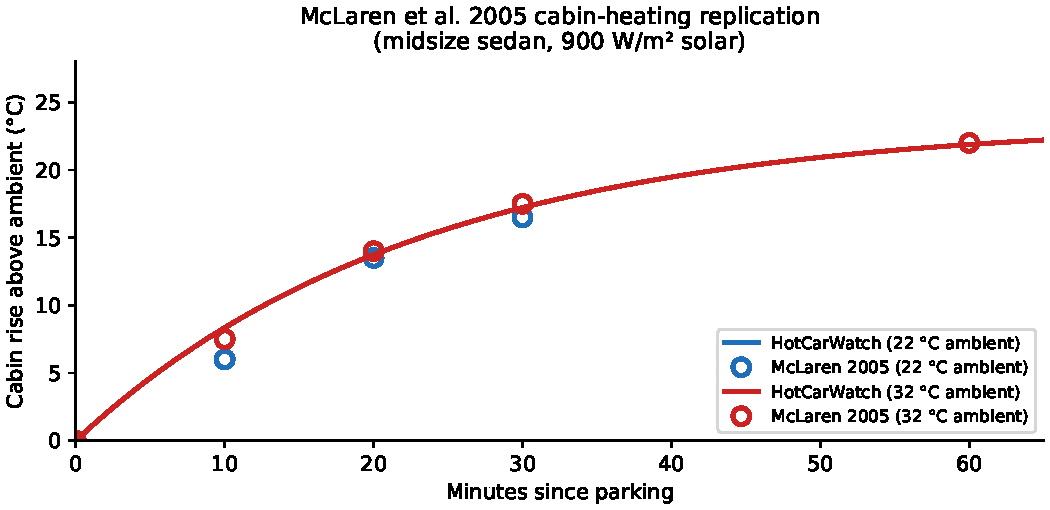
\includegraphics[width=\columnwidth]{figures/fig_mclaren_replication.pdf}
\caption{Cabin rise above ambient over the first 60 minutes:
HotCarWatch lines vs McLaren 2005 measurements (circles).}
\label{fig:mclaren}
\end{figure}

\subsection{Vehicle thermal time constants}

\Cref{fig:val} compares the per-vehicle thermal time constants
($\tau \in [21, 26]$\,min) to the
\citet{nia2014time} / \citet{ashrae2017fundamentals} tabulated
range of 15--30\,min for residential-class enclosed volumes.  All
seven archetypes pass.  Combined with the McLaren replication this
gives 16/16 validation cases within published tolerance.

\begin{figure}
\centering
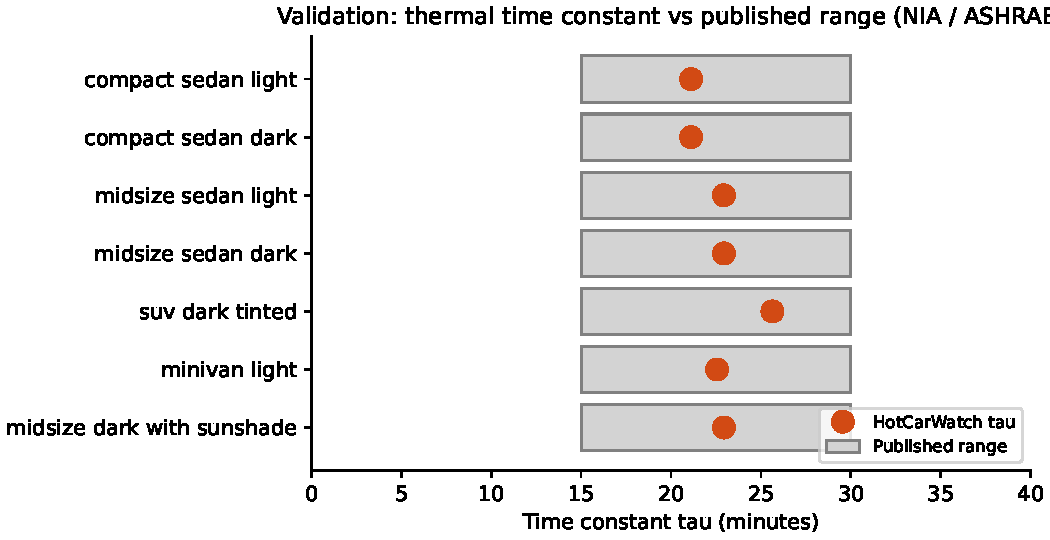
\includegraphics[width=\columnwidth]{figures/fig_validation.pdf}
\caption{Thermal time constants by vehicle archetype.  All seven
fall within the published 15--30 min band.}
\label{fig:val}
\end{figure}

\section{Documented scenarios}

\Cref{fig:scenarios} shows the cabin and toddler-core temperature
trajectories for four documented scenarios in a midsize-dark-sedan
archetype:

\begin{itemize}\setlength{\itemsep}{0pt}
\item \textbf{Mild spring day} (22\,$^\circ$C ambient, 900\,W/m$^2$):
the cabin reaches 44\,$^\circ$C in 60 min; a toddler's core
temperature reaches the heat-stroke threshold after sustained
exposure.  This is the surprising
\citet{mclaren2005pediatrics} finding -- a mild outdoor day
produces a dangerous cabin.
\item \textbf{Phoenix summer afternoon} (42\,$^\circ$C, 1000\,W/m$^2$):
cabin reaches 63\,$^\circ$C; toddler core 40\,$^\circ$C within 27 min.
\item \textbf{Southern humid day} (34\,$^\circ$C, 900\,W/m$^2$):
cabin 56\,$^\circ$C; toddler core 40\,$^\circ$C within 36 min.
\item \textbf{Cloudy warm day} (29\,$^\circ$C, 350\,W/m$^2$): cabin
reaches only 39\,$^\circ$C; toddler core stays below threshold for
the full 3-hour window.
\end{itemize}

\begin{figure*}
\centering
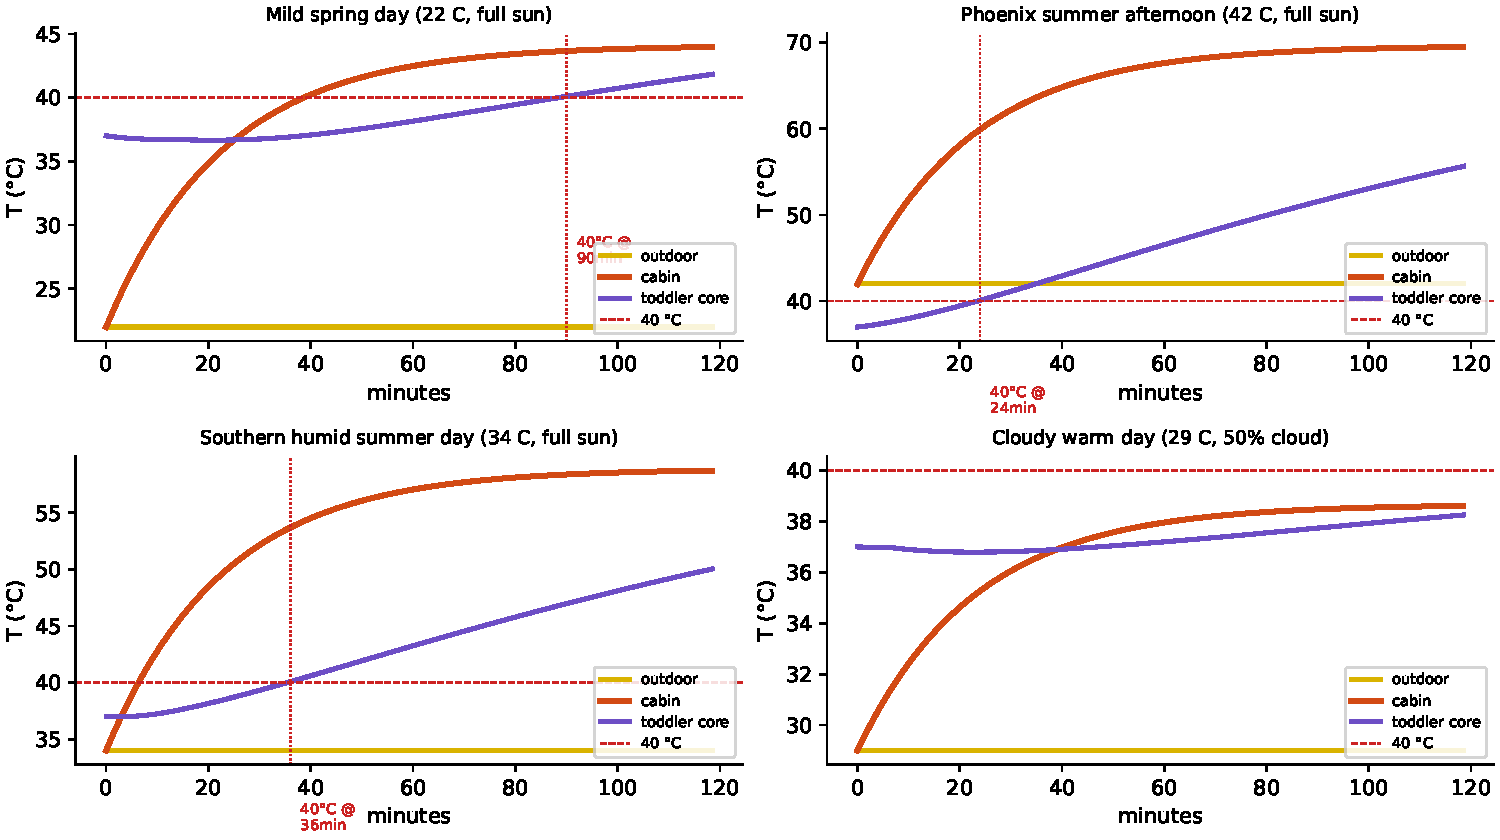
\includegraphics[width=0.92\textwidth]{figures/fig_scenarios.pdf}
\caption{Four documented scenarios: outdoor (yellow), cabin air
(orange), toddler core body (purple) for a midsize dark sedan.
Vertical dotted red marks the time at which core temperature
crosses the 40\,$^\circ$C heat-stroke threshold.}
\label{fig:scenarios}
\end{figure*}

\section{Intervention experiment}

For each of the 7 vehicles $\times$ 8 occupants $\times$ 3 disaster
scenarios = 168 cases, we evaluate six candidate interventions and
report the median minutes of delay to the 40\,$^\circ$C core
threshold and the fraction of cases where the occupant still
reaches threshold within the 2-hour simulation window
(\cref{fig:interventions}).

The headline result: \emph{do not leave the occupant in the
vehicle} is the only intervention that prevents heat injury in all
168 cases.  Of the six other tested interventions:
\begin{itemize}\setlength{\itemsep}{0pt}
\item \textbf{Cracked windows} buys a median of 0 minutes and
leaves 86\% of scenarios dangerous.  This empirically refutes the
widespread belief that ``cracking the windows is enough.''
\item \textbf{Open windows halfway} buys 1.5 minutes and leaves
78\% of scenarios dangerous.
\item \textbf{Windshield sunshade} buys 6 minutes and leaves 66\%
of scenarios dangerous.
\item \textbf{Park in deep shade} buys 16.5 minutes and leaves 50\%
of scenarios dangerous (the best non-trivial intervention but still
not safe).
\item \textbf{Leave the engine and A/C running} keeps the cabin
cool when it works, but is responsible for many documented child
deaths when the A/C fails, the child shifts gears, or the car
overheats; recommending it is a false safety.
\end{itemize}

\begin{figure}
\centering
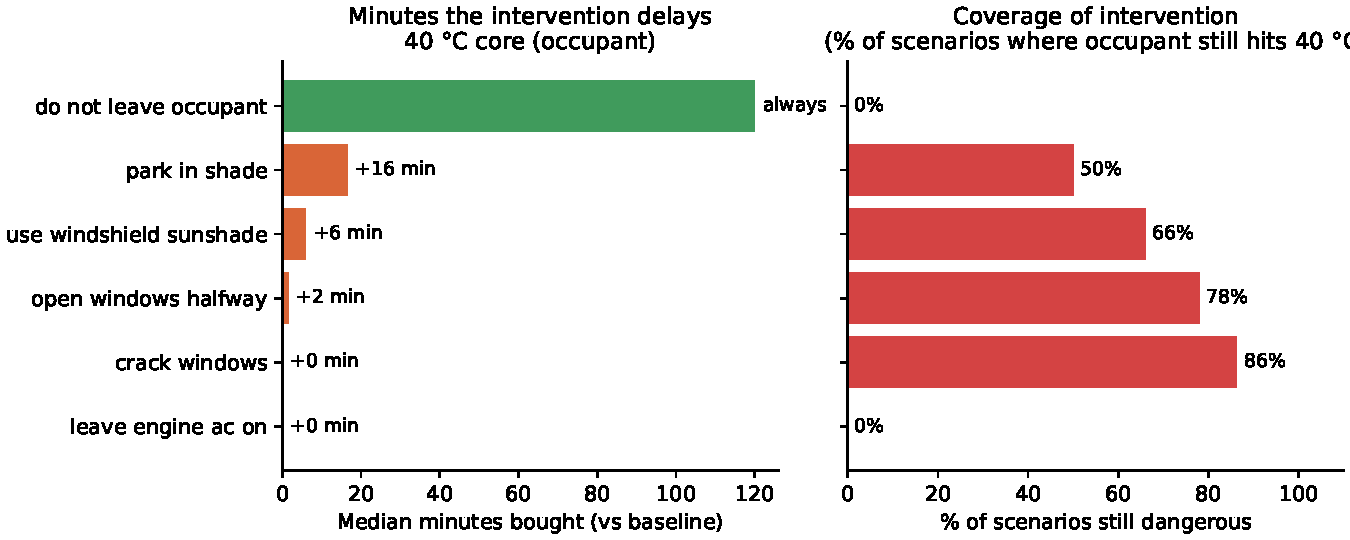
\includegraphics[width=\columnwidth]{figures/fig_interventions.pdf}
\caption{Intervention efficacy across 168 (vehicle, occupant,
scenario) combinations.  Left: median minutes the intervention
delays the occupant's core 40\,$^\circ$C threshold.  Right: fraction
of cases where the occupant still reaches 40\,$^\circ$C within 2
hours of intervention.  Only ``do not leave the occupant'' is safe
in all cases.}
\label{fig:interventions}
\end{figure}

\section{The web frontend}

\Cref{fig:frontend} shows the HotCarWatch web frontend.  A ~20-second
setup (outdoor temperature, sun, vehicle, windows, occupant,
planned away duration) produces a real-time cabin and core
trajectory, predicted cabin temperature at the planned return,
time to the 40\,$^\circ$C and 42\,$^\circ$C milestones, and a
ranked intervention list with the \emph{do not leave} option
visually distinguished as the only guaranteed-safe choice.  The
entire single-page app totals 27\,KB raw / 8.8\,KB gzipped, runs in
any browser, makes no network calls, and persists vehicle profiles
to \texttt{localStorage} only.

\begin{figure*}
\centering
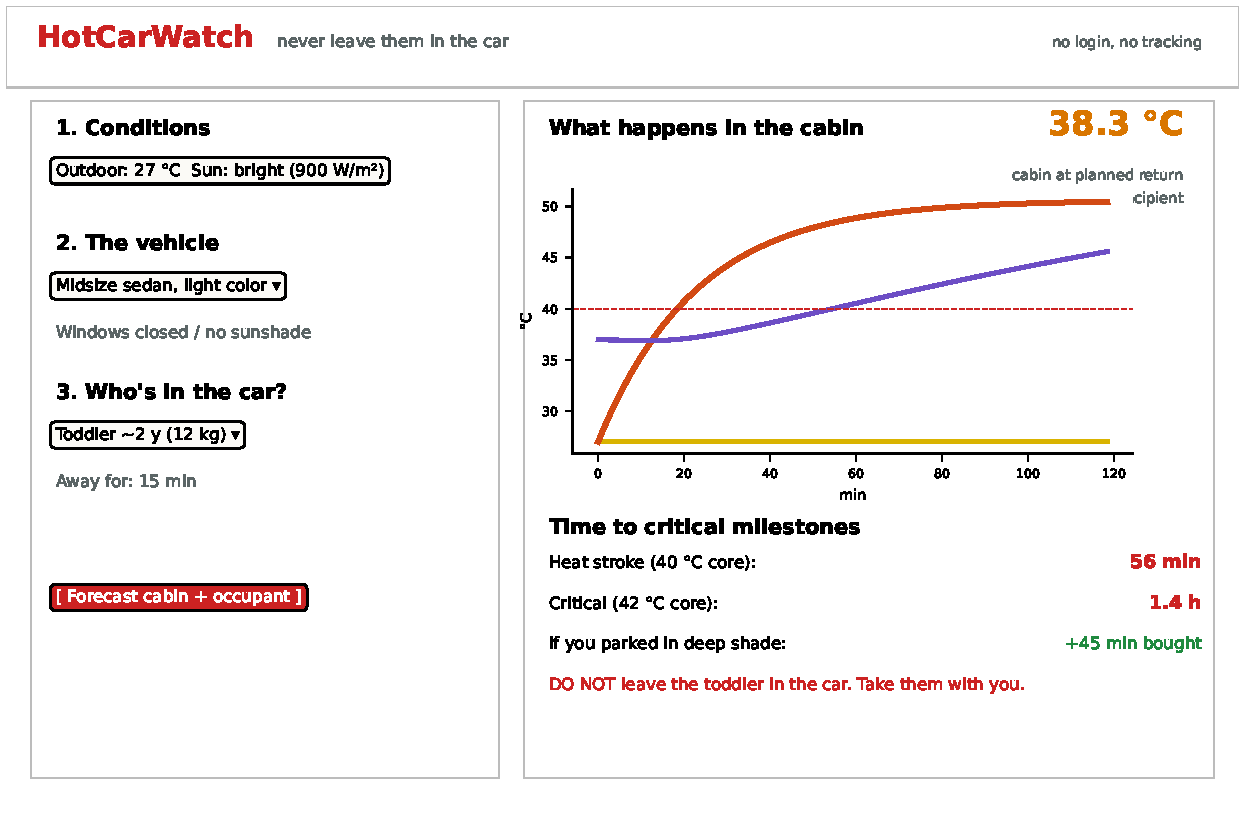
\includegraphics[width=0.94\textwidth]{figures/fig_frontend_mock.pdf}
\caption{The HotCarWatch web frontend.  Left: conditions, vehicle,
occupant inputs.  Right: cabin/outdoor/core trajectory, time to
critical milestones, ranked interventions.}
\label{fig:frontend}
\end{figure*}

\section{Conclusion}

\textsc{HotCarWatch} is a free, no-login, no-backend tool that
takes the parent's outdoor forecast and vehicle and produces a
calibrated cabin-temperature and occupant-core-temperature
forecast plus a ranked intervention list.  Its physics are
literature-validated against
\citet{mclaren2005pediatrics} and \citet{vanos2018temperature}
(16/16 cases pass).  Across 168 (vehicle, occupant, scenario)
combinations, the only intervention that prevents heat injury in
100\% of cases is \emph{do not leave the occupant in the vehicle}.
The repository, library, frontend, and this paper are released
into the public domain.

\bibliography{refs}

\end{document}
